\documentclass[12pt]{book}
\usepackage[margin=.85in]{geometry} % for MARGIN
\usepackage[many]{tcolorbox}    	% for COLORED BOXES (tikz and xcolor included)


\usepackage{multicol}   
\usepackage{enumerate}
\usepackage[shortlabels]{enumitem}
\usepackage{varwidth}
\usepackage{tasks}
\usepackage[export]{adjustbox}
\usepackage[dvipsnames]{xcolor}

\usepackage{titleps}
\usepackage{setspace}               % for LINE SPACING
\usepackage[⟨options⟩]{fancyhdr}
\usepackage{enumitem}
\setlist{nosep}
\usepackage{tikz}
\usepackage{pgfplots}
\pgfplotsset{compat=1.5.1}
\usetikzlibrary{datavisualization}
\usetikzlibrary{datavisualization.formats.functions}

\newcommand{\D}{\displaystyle}


\setlength\parindent{0pt}   % killing indentation for all the text
\setstretch{1.3}            % setting line spacing to 1.3
\setlength\columnsep{0.25in} % setting length of column separator
\pagestyle{fancy}           % setting pagestyle to be headings

\usepackage[]{titlesec}

\fancyhead[L]{Math V04 - College Algebra}
\fancyhead[R]{Christina Papazacharioudakis}

\tcbset{
    sharp corners,
    colback = white,
    before skip = 0.2cm,    % add extra space before the box
    after skip = 0.5cm      % add extra space after the box
}                           % setting global options for tcolorbox

    \newtcolorbox{boxR}{
    fontupper = \color{black}, % font color
    boxrule = 1.5pt,
    colframe = black,
    rounded corners,
    arc = 5pt   % corners roundness
}

\definecolor{ballblue}{rgb}{0.13, 0.67, 0.8}

\begin{document}



\begin{comment}
Name: \underline{\hspace{100mm}}
\vspace{20mm}
  \centerline{\Large \textbf{Chapter 2: Equations and Inequalities} } 

{\large
\begin{center}
\begin{varwidth}{\textwidth}
\begin{enumerate}[2.1]
    \item The Regular Coordinate System and Graphs
    \item Linear Equations in One Variable
    \item Models and  Applications (Skipping)
    \item Complex Numbers
    \item Quadratic Equations
    \item Other Types of Equations
    \item Linear Inequalities and Absolute Value Inequalities
\end{enumerate}
\end{varwidth}
\end{center}

}
\newpage  
\end{comment}

\textbf{{\Large 3.3 Rates of Change and Behavior of Graphs}}
\vspace{5mm}



{\large \textbf{Finding the Average Rate of Change of a Function}}
\vspace{3mm}

Some motivation:

Every year, we see a fluctuation of gasoline prices. The table below lists the average cost, in dollars, of gasoline per gallon from $2005-2012$. We can think of the cost of gasoline as a function of the year. 



\vspace{5mm}

\centerline{
\begin{tabular}{|c|c|c|c|c|c|c|c|c|} 
 \hline
$y$ & $2005$ & $2006$ & $2007$ & $2008$ & $2009$ & $2010$ & $2011$ & $2012$   \\
 \hline
 $C(y)$ & $2.31$ & $2.62$ & $2.84$ & $3.30$ & $2.41$ & $2.84$ & $3.58$ & $3.68$   \\
 \hline
\end{tabular}}

\vspace{5mm}


If we were interested only in how the gasoline prices changed between $2005$ and $2012$, we could compute that the cost per gallon had increased from $\$2.31$ to $\$3.68$, an increase of $\$1.37$. 

\vspace{5mm}

While this is interesting, it might be more useful to look at how much the price changed with respect to how many years have gone by (how much time went by for that change in price to happen?). If we consider the gas price change over $7$ years, this gives us the \textbf{average rate of change} of gas prices per year:

$$ \frac{\text{change in price}}{\text{change of time}} = \frac{C(2012) - C(2005)}{2012 - 2005 \text{ years }}  = \frac{\$3.68 - \$2.31}{2012 - 2005 \text{ years }} =  \frac{\$1.37}{7 \text{ years }} \approx 0.196 \text{ dollars per year}$$

\vspace{3mm}
On average, the price of gas increased by about $19.6$¢ per year from 2005 to 2012.
\vspace{5mm}

Formalizing this idea, we have: 
\begin{align*}
    \text{Average rate of change} &= \frac{\text{Change in output}}{\text{Change in input}} \\
    & = \frac{\Delta C}{\Delta y} &&\text{Greek letter $\Delta$ (delta) signifies change in quantity} \\
    & = \frac{C_2 -C_1}{y_2-y_1} \\
    & = \frac{C(y_2)-C(y_1}{y_2-y_1}
\end{align*}
 Where years, $y$, was our input, and cost, C, was our output. 

\newpage

\begin{boxR}
    \textbf{Rate of Change of a Function}
    \vspace{1mm}
    \hline
    \vspace{2mm}
The \textbf{average rate of change of a function} is the change in the output values divided by the change in the input values.

$$ \frac{\Delta y}{\Delta x} = \frac{f(x_2) - f(x_1)}{x_2-x_1}$$

Here, \textbf{total change of a function} is defined as $ \D \Delta y = f(x_2) - f(x_1)$
\end{boxR}

\begin{boxR}
    \textbf{How To}
    \vspace{1mm}
    \hline
    \vspace{2mm}
   \textbf{ Given the value of a function at different points, calculate the average rate of change of a function from $x_1$ to $x_2$.}
   \begin{enumerate}
       \item Calculate the total change of the function, $\Delta y = f(x_2)-f(x_1)$.
       \item Calculate $\Delta x = x_2-x_1$.
       \item Find the ratio $\frac{\Delta y}{\Delta x}$.
   \end{enumerate}
\end{boxR}

\underline{\textbf{Example 2 - Computing Average Rate of Change from a Graph.}}

Given the function $g(t)$, find the average rate of change of $g(t)$ on the interval $[-1, 2]$. This interval means that $t$ starts at $-1$ and ends at $2$.
\\

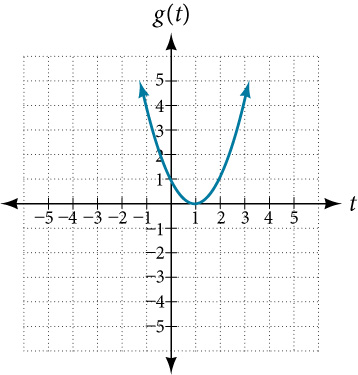
\includegraphics[scale=1.3]{Chapter 3/3.3-figure1.jpeg}

\newpage


\underline{\textbf{Example 4 - Computing Average Rate of Change for a Function Expressed as a Formula}}
\vspace{1mm}

Calculate the average rate of change of $\D f(x)=x^2 - \frac{1}{x}$ in the interval $[2,4]$.

\vspace{80mm}

{\large \textbf{Using a Graph to Determine Where a Function is Increasing, Decreasing, or Constant}}
\vspace{3mm}

As part of exploring how functions can change, we can identify intervals over which the function is increasing or decreasing. Let's take a look at a visual:

\centerline{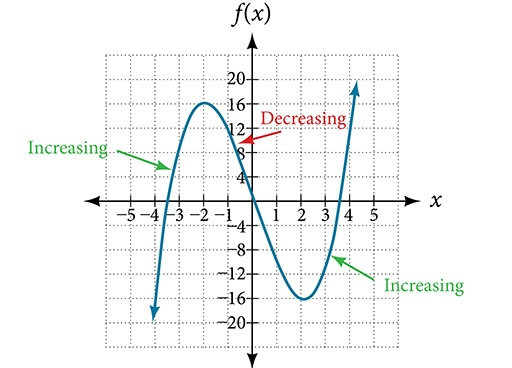
\includegraphics[scale=.6]{Chapter 3/3.3-figure2.jpeg}}

\\


Reading the graph (or $x$ values) from left to right:
\\

\centerline{
\textcolor{ForestGreen}{$\D f(-4) < f(-3)$ \hspace{5mm}}
\textcolor{Maroon}{$\D f(-1) > f(1)$  \hspace{5mm}}
\textcolor{ForestGreen}{$\D f(3) < f(4)$ } }
\newpage



 \begin{comment}
     \underline{\textbf{Example 2 - Finding the Domain of a Function as a Set of Ordered Pairs}}
   
    Find the domain and range of the following function: $$\{ (2,10), (3,10), (4,20), (5,30), (6,40)\}$$
    \vspace{5mm}
    Domain: 
   
    Range: 
 \end{comment}  

\begin{boxR}
    \textbf{Increasing and Decreasing Behavior of a Function}
    \vspace{1mm}
    \hline
    \vspace{2mm}
A function  \textbf{$f(x)$ is increasing} on an interval $I$ if 
$$ f(x_1) < f(x_2) \text{ whenever } x_1 < x_2 \text{ in } I$$ 
 

A function  \textbf{$f(x)$ is decreasing} on an interval $I$ if 
$$ f(x_1) > f(x_2) \text{ whenever } x_1 < x_2 \text{ in } I$$ 
\end{boxR}

\vspace{1mm}

\underline{\textbf{Example 7 - Finding intervals of Increase and Decrease of a Graph}}

Given the graph of $p(t)$, identify the intervals where $p(t)$ increases and decreases.

\begin{multicols}{2}
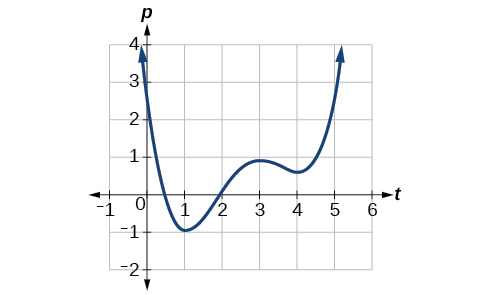
\includegraphics[scale=1.3]{Chapter 3/3.3-figure3.jpeg}
\\

Increasing: 
\\
\vspace{5mm}

Decreasing: 
\end{multicols}

\vspace{5mm}

Where is the function neither increasing nor decreasing? 
\\

A \textbf{local maximum} occurs when we see a peak in our graph. What is the local maximum? Where does it occur? 
\\

A \textbf{local minimum} occurs when we see a valley in our graph. What are the local minimums? Where do they occur?



\newpage



\begin{boxR}
    \textbf{Local Minima and Local Maxima}
    \vspace{1mm}
    \hline
    \vspace{2mm}
The number $f(c)$ is a 
\begin{itemize}
    \item \textbf{local maximum} of $f$ if $f(c) \geq f(x)$ when $x$ is near $c$.
     \item \textbf{local minimum} of $f$ if $f(c) \leq f(x)$ when $x$ is near $c$.
\end{itemize}
\end{boxR}
\vspace{1mm}


\underline{\textbf{Example 9 - Find the Local Maxima and Minima from the Graph}}

Find all local maxima and minima for the graph of $f$.

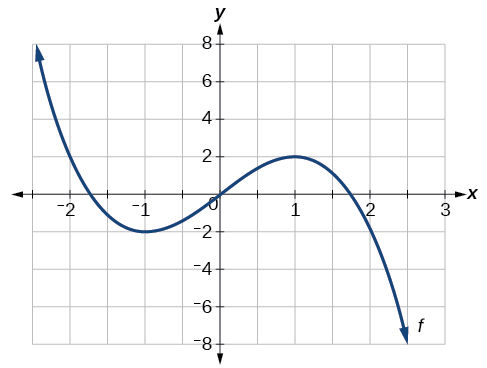
\includegraphics[scale=.85]{Chapter 3/3.3-figure4.jpeg}

\vspace{3mm}
{\large \textbf{Analyzing the Toolkit Functions for Increasing or Decreasing Intervals}}

We will now return to our toolkit functions and discuss their graphical behavior.
\\

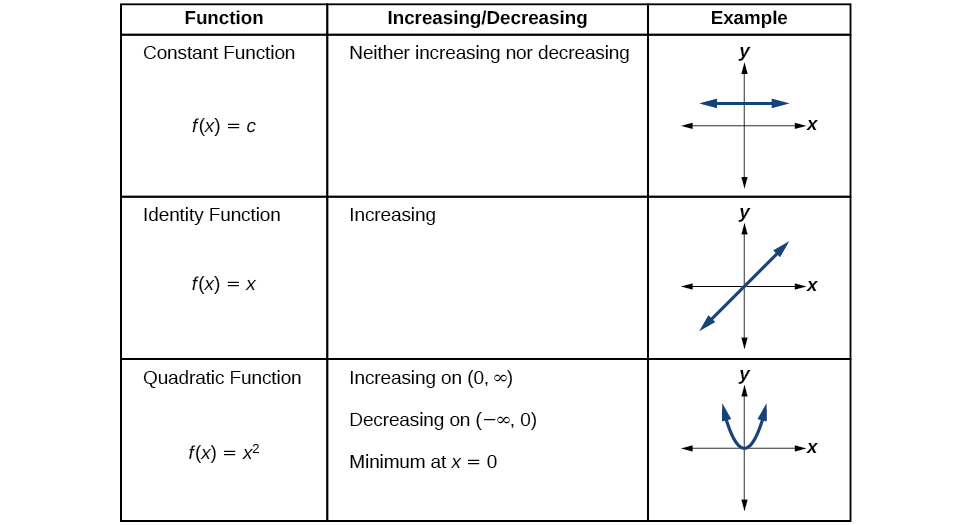
\includegraphics[scale=1]{Chapter 3/3.3-figure5.jpeg}

\newpage


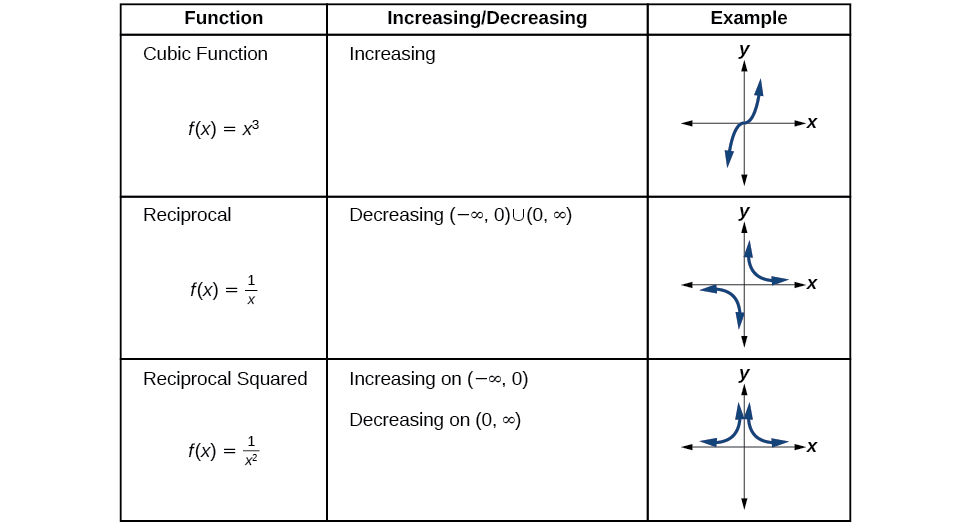
\includegraphics[scale=1]{Chapter 3/3.3-figure6.jpeg}

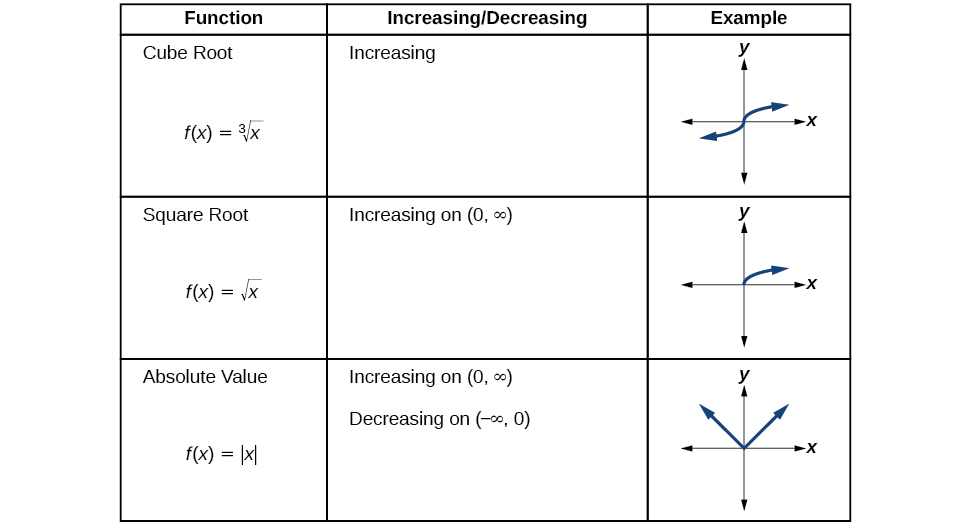
\includegraphics[scale=1]{Chapter 3/3.3-figure7.jpeg}


\newpage


\textbf{\large Use a Graph to Locate the Absolute Maximum and Absolute Minimum}

We now look at finding the largest possible $y$ value of a function and the smallest possible $y$ value of a function throughout its entire domain. The $y$ value of the highest and lowest points of $f$ are called the \textbf{ absolute maximum} and the \textbf{absolute minimum}, respectively.
\\ 

\centerline{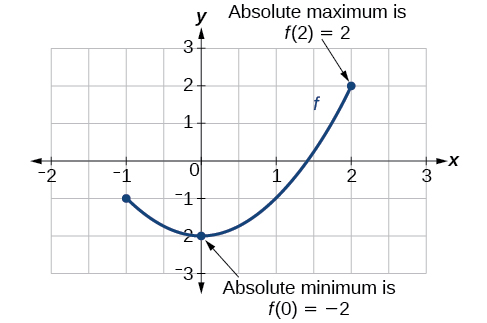
\includegraphics[height=50mm, width=70mm]{Chapter 3/3.3-figure8.jpeg}}

\vspace{5mm}


\begin{boxR}
    \textbf{Absolute Maxima and Minima}
    \vspace{1mm}
    \hline
    \vspace{2mm}
    Suppose that $c$ is some number in the domain of $f$. Then $f(c)$ is the
    \begin{itemize}
        \item \textbf{absolute maximum} value of $f$ if $f(c) \geq f(x)$ for every $x$ in the domain of $f$.
        \item \textbf{absolute maximum} value of $f$ if $f(c) \leq f(x)$ for every $x$ in the domain of $f$.
    \end{itemize}

\end{boxR}

\vspace{5mm}


\underline{\textbf{Example 10 - Find the Absolute Maxima and Minima from a Graph}}

Find the absolute maxima and minima for the function $f$ shown below. 

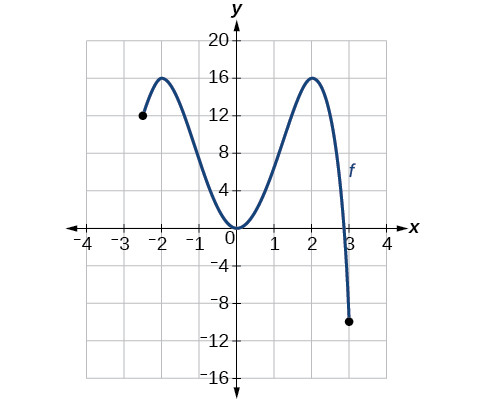
\includegraphics[scale=1]{Chapter 3/3.3-figure9.jpeg}

\newpage


\textbf{{\Large 3.4 Composition of Functions}}
\vspace{3mm}

Two functions $f$ and $g$ can be combined to form new functions $f+g$, $f-g$, $fg$, and $f/g$ in a similar way to the way we add, subtract, multiply, and divide real numbers.

\vspace{5mm}



\begin{boxR}
    \textbf{Sum, Difference, Product, and Quotient Functions}
    \vspace{1mm}
    \hline
    \vspace{2mm}
Given two functions $f$ and $g$, the following functions are defined as follows: 

\vspace{2mm}
\textbf{Sum Function:} $\D (f+g)(x)=f(x) + g(x)$
    \vspace{3mm}
    
\textbf{Difference Function:} $\D (f-g)(x)=f(x) - g(x)$
    \vspace{3mm}
    
\textbf{Product Function:}  $\D (fg)(x) = f(x)g(x)$
    \vspace{3mm}
    
    \textbf{Quotient Function:}
 $\D (f/g)(x) = \frac{f(x)}{g(x)} \hspace{3mm}, g(x)\neq 0$   


\end{boxR}


\underline{\textbf{Example 1 - Performing Algebraic Operations on Functions}}
\vspace{3mm}

Find and simplify the functions $(f-g)(x)$ and $(f/g)(x)$ given that $f(x)=x^2-1$ and $g(x)=x-1$.
\vspace{1mm}
\newpage

{\large \textbf{Create a Function by Composition of Functions}}

Performing algebraic operations on functions (adding, subtracting, multiplying, and dividing) created new functions. We can also create functions by composing them. This process includes taking the output of one function and using it as the input of another function. The resulting function is known as a \textbf{composite function}. We represent this combination by the following notation:
$$(f \circ g)(x) = f(g(x))$$
This reads ``$f$ of $g$ of $x$".
\\

For example, if $f(x) = x^2$ and $g(x)=x+2$ then,
\\

   $f(g(x))= $

   \vspace{50mm}




Note that in many cases, $f(g(x)) \neq g(f(x))$. They are different functions. Let's take a look:
\\

   $g(f(x))= $

   \vspace{50mm}

\newpage


\begin{boxR}
    \textbf{Composition of Functions}
    \vspace{1mm}
    \hline
    \vspace{2mm}
   When the output of one function is used as the input of another, we call the entire operation a composition of functions. This action defined a composite function, which we write as:
   $$ (f \circ g)(x) = f(g(x))$$

 The domain of $f \circ g$ is the set of all $x$ in the domain of $g$ such that $g(x)$ is also in the domain of $f$. 
\end{boxR}
{\large \textbf{Evaluating Composite Functions}}
\vspace{1mm}

Once we compose a new function from two existing functions, we need to be able to evaluate it for any input in its domain. We evaluate the inner function first, and then use its output as the input of the outer function.

\centerline{ 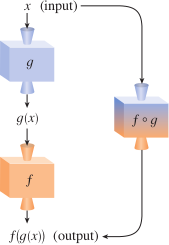
\includegraphics[scale=.9]{Chapter 3/3.4-figure1.png} }

\vspace{1mm}
\underline{\textbf{Example 5 - Using a Table to Evaluate a Composite Function}}

Find $f(g(3))$ and $g(f(3))$ using the table.
\\

\begin{tabular}{ |c|c|c| } 
 \hline
 $x$ & \hspace{3mm} $f(x) \hspace{3mm}$ & \hspace{3mm} $g(x)$ \hspace{3mm} \\
 \hline
 $1$ & $6$ & $3$ \\
 \hline
 $2$ & $8$ & $5$ \\
 \hline
 $3$ & $3$ & $2$ \\
 \hline
  $4$ & $1$ & $7$ \\
 \hline
\end{tabular}
\newpage


\textbf{Evaluating Composite Functions Using Graphs}



\begin{boxR}
    \textbf{How To}
    \vspace{1mm}
    \hline
    \vspace{2mm}
   \textbf{Given a composite function and graphs of its individual functions, evaluate it using the information provided by the graphs.}
   \begin{enumerate}
       \item Locate the given input to the inner function on the $x$-axis of its graph.
       \item Read off the output of the inner function from the  $y$-
       axis of its graph.
       \item Locate the inner function output on the $x$-axis of the graph of the outer function.
       \item Read the output of the outer function from the  $y$-axis of its graph. This is the output of the composite function.
   \end{enumerate}
\end{boxR}

  
\underline{\textbf{Example 6 - Using a Graph to Evaluate a Composite Function}}

Evaluate $f(g(1))$ and $g(f(2))$.
\\

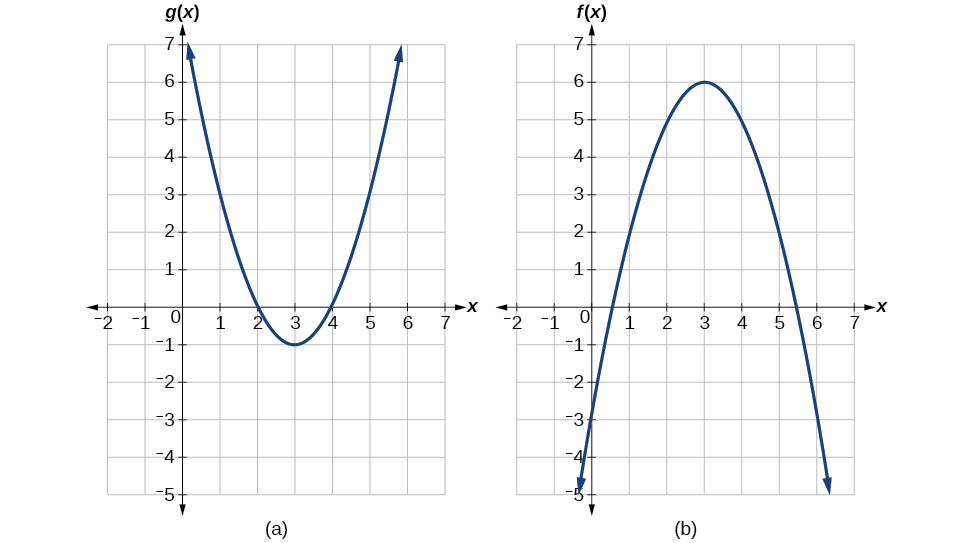
\includegraphics[scale=.8]{Chapter 3/3.4-figure2.jpeg}

 \newpage



{\large \textbf{Evaluating Composite Functions Using Formulas}}


When evaluating a composite function using formulas, the process of working from the inside out remains the same. 

\vspace{3mm}

\begin{boxR}
    \textbf{How To}
    \vspace{1mm}
    \hline
    \vspace{2mm}
    \textbf{Given a formula for a composite function, evaluate the function.}
    \begin{enumerate}
        \item Evaluate the inside function using the input value or variable provided.
        \item Use the resulting output as the input to the outside function.
    \end{enumerate}
\end{boxR}
\vspace{3mm}



\underline{\textbf{Example 7 - Evaluating a Composition of Functions Expressed as Formulas}}

Given $f(t)=t^2-t$ and $h(x)= 3x+2$, evaluate $f(h(1))$.

\newpage

{\large \textbf{Finding the Domain of a Composite Function}}

As mentioned in the beginning of this section, the domain of $f \circ g$ depends on both the domain of $g$ and the domain of $f$:
\\

\begin{boxR}
    \textbf{Domain of a Composite Function}
    \vspace{1mm}
    \hline
    \vspace{2mm}
    The domain of a composite function $f(g(x))$ is the set of those inputs $x$ in the domain of $g$ for which $g(x)$ is also in the domain of $f$.
\end{boxR}

\begin{boxR}
    \textbf{How To}
    \vspace{1mm}
    \hline
    \vspace{2mm}
    \textbf{Given a function composition $f(g(x))$ determine its domain.}
    \begin{enumerate}
        \item Find the domain of $g$.
        \item Find the domain of $f$
        \item Find the inputs $x$ in the domain of $g$ such that $g(x)$ is in the domain of $f$. That is, exclude $x$ values from the domain of $g$ for which $g(x)$ is not in the domain of $f$.
    \end{enumerate}
\end{boxR}

\underline{\textbf{Example 8 - Finding the Domain of a Composite Function}}
\vspace{2mm}

Find the domain of $(f \circ g)(x) = f(g(x))$ where 
$\D f(x) = \frac{5}{x-1}$ and $\D g(x) = \frac{4}{3x-2}$.

\newpage
{\large \textbf{Decomposing a Composite Function into its Component Functions}}
\vspace{3mm}

Given a composite function, we may want to write it as a composition of two simpler functions. Let's take a look:
\\

\underline{\textbf{Example 10 - Decomposing a Function}}
\vspace{2mm}

Write $\D h(x) = \sqrt{5-x^2}$ as the composition of two functions. 
\newpage






\end{document}


